\documentclass[sigchi, review]{acmart}

\usepackage{booktabs} % For formal tables


% Copyright
%\setcopyright{none}
%\setcopyright{acmcopyright}
%\setcopyright{acmlicensed}
%\setcopyright{rightsretained}
%\setcopyright{usgov}
%\setcopyright{usgovmixed}
%\setcopyright{cagov}
\setcopyright{licensedcagov}
%\setcopyright{cagovmixed}
%\setcopyright{licensedothergov}

% DOI
\acmDOI{10.475/123_4}

% ISBN
\acmISBN{123-4567-24-567/08/06}

%Conference
\acmConference[WOODSTOCK'97]{ACM Woodstock conference}{July 1997}{El
  Paso, Texas USA}
\acmYear{1997}
\copyrightyear{2016}

\acmPrice{15.00}


\begin{document}
\title{Co-designing Mobile Online Safety Applications with Children }
\titlenote{Produces the permission block, and
  copyright information}
\subtitlenote{The full version of the author's guide is available as
  \texttt{acmart.pdf} document}

\author{Brenna McNally}
\authornote{Dr.~Trovato insisted his name be first.}
\orcid{1234-5678-9012}
\affiliation{%
  \institution{Human-Computer Interaction Lab  }
  \institution{College of Information Studies, College Park}
}
\email{trovato@corporation.com}

\author{Priya Kumar}
\authornote{The secretary disavows any knowledge of this author's actions.}
\affiliation{%
  \institution{Human-Computer Interaction Lab }
  \institution{College of Information Studies, College Park}
}
\email{webmaster@marysville-ohio.com}

\author{ Chelsea Hordatt}
\authornote{This author is the
  one who did all the really hard work.}
\affiliation{%
  \institution{Human-Computer Interaction Lab  }
  \institution{College of Information Studies, College Park}
}
\email{larst@affiliation.org}

\author{ Matthew Louis Mauriello}
\affiliation{%
  \institution{Human-Computer Interaction Lab }
  \institution{Department of Computer Science University of Maryland, College Park}
}
\author{Shalmali Naik}
\affiliation{%
 \institution{Human-Computer Interaction Lab }
  \institution{College of Information Studies, College Park}
}

\author{ Leyla Norooz}
\affiliation{%
  \institution{Human-Computer Interaction Lab }
  \institution{College of Information Studies, College Park}
}

\author{ Alazandra Shorter}
\affiliation{%
  \institution{Human-Computer Interaction Lab }
  \institution{College of Information Studies, College Park}
}
\email{cpalmer@prl.com}

\author{Evan Golub}
\affiliation{
   \institution{Human-Computer Interaction Lab }
  \institution{Department of Computer Science University of Maryland, College Park}
}
\email{jsmith@affiliation.org}

\author{Allison Druin}
\affiliation{
   \institution{Human-Computer Interaction Lab }
  \institution{College of Information Studies, College Park}
}
\email{jpkumquat@consortium.net}

% The default list of authors is too long for headers.
\renewcommand{\shortauthors}{B. Trovato et al.}


\begin{abstract}
Parents use mobile monitoring software to observe and restrict their children’s activities in order to minimize the risks associated with Internet-enabled mobile devices. As children are stakeholders in such technologies, recent research has called for their inclusion in its design process. To investigate children’s perceptions of parental mobile monitoring technologies and explore their interaction preferences, we held two co-design sessions with 12 children ages 7-12. Children first reviewed and redesigned an existing mobile monitoring application. Next, they designed ways children could use monitoring software when they encounter mobile risks (e.g., cyberbullying, inappropriate content). Results showed that children acknowledged safety needs and accepted certain parental controls. They preferred and designed controls that emphasized restriction over monitoring, taught risk coping, promoted parent-child communication, and automated interactions. Our results benefit designers looking to develop parental mobile monitoring technologies in ways that children will both accept and can actively benefit from. 
\end{abstract}

%
% The code below should be generated by the tool at
% http://dl.acm.org/ccs.cfm
% Please copy and paste the code instead of the example below.
%
\begin{CCSXML}
<ccs2012>
 <concept>
  <concept_id>10010520.10010553.10010562</concept_id>
  <concept_desc>Computer systems organization~Embedded systems</concept_desc>
  <concept_significance>500</concept_significance>
 </concept>
 <concept>
  <concept_id>10010520.10010575.10010755</concept_id>
  <concept_desc>Computer systems organization~Redundancy</concept_desc>
  <concept_significance>300</concept_significance>
 </concept>
 <concept>
  <concept_id>10010520.10010553.10010554</concept_id>
  <concept_desc>Computer systems organization~Robotics</concept_desc>
  <concept_significance>100</concept_significance>
 </concept>
 <concept>
  <concept_id>10003033.10003083.10003095</concept_id>
  <concept_desc>Networks~Network reliability</concept_desc>
  <concept_significance>100</concept_significance>
 </concept>
</ccs2012>
\end{CCSXML}

\ccsdesc[500]{Computer systems organization~Embedded systems}
\ccsdesc[300]{Computer systems organization~Redundancy}
\ccsdesc{Computer systems organization~Robotics}
\ccsdesc[100]{Networks~Network reliability}

\begin{teaserfigure}
  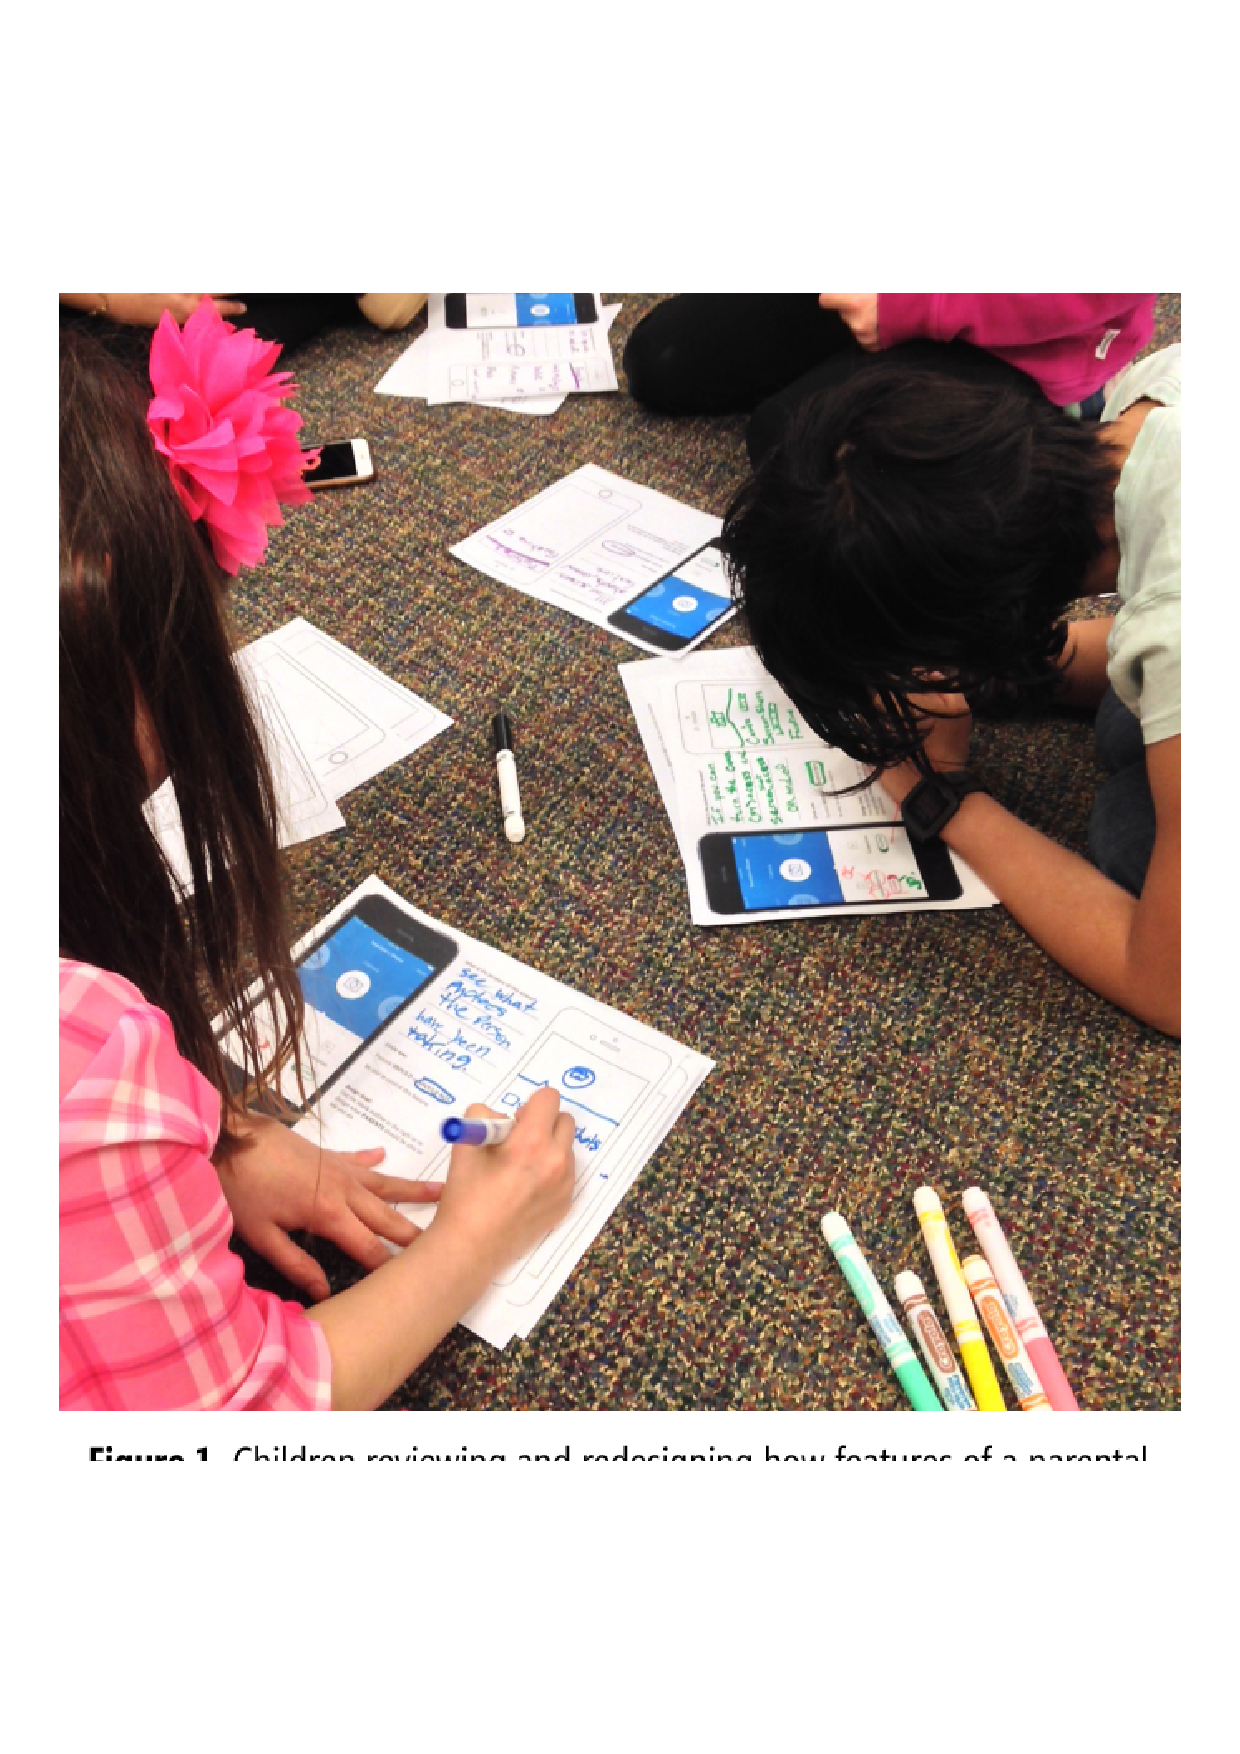
\includegraphics[width=\textwidth]{Children}\Description{A
    baseball field}
  \caption{This is a teaser}
  \label{fig:teaser}
\end{teaserfigure}


\maketitle

\section{Introduction}
 Mobile technologies have made their way into our homes, into our lives, and into children’s pockets 
Mobile devices provide children a convenient method to communicate with family and friends, 
earn parental trust, and learn responsibility . They also offer opportunities for safety , 
learning , and entertainment .  Risks related to children’s Internet access include content threats , 
contact threats , conduct threats , and computer threats .We coded the application features children 
designed using the Teen Online Safety Strategies (TOSS) Framework 

\section{Process}
90 minutes,introduced to the design prompt and activity, small groups of 2-3 children 
and 1-2 adults were formed to complete the design tasks. 
After the design activity, the groups presented their ideas to the rest of the team. 

\section{Participants}
all 12 children (ages 7-12, 8 female) completed the survey and redesign activity that was conducted at both design sessions

\section{Participants}



\cite{mcnally2018co}
\cite{chaves2018single}
\cite{robinson2018make}
 

\bibliographystyle{ACM-Reference-Format}
\bibliography{reference}

\end{document}
